\documentclass[
	spanish,
	9pt,
	xcolor=table,
	handout,
	aspectratio=1610,
	%ignorenonframetext
]{beamer}

\usepackage[spanish]{babel}
\usepackage[
	cursointroductorio,
	fullpagenumbering
]{dunestyle-beamer}
%\usepackage{svg}
%\graphicspath{{./images}}
\usepackage{booktabs}
\usepackage{longtable}

\usepackage[backend=biber,style=numeric, defernumbers=true, sorting=ynt,maxbibnames=4,maxcitenames=4]{biblatex}
\addbibresource{dune-webinar-references.bib}

\title{
	Una introducción a la caja de herramientas DUNE en \texttt{C++}/\texttt{Python} para la solución de modelos matemáticos
}
\subtitle{
	Parte I:
	\lstinline{bash}
}

\author{}
\institute[]
{
	\noindent
	Practique los ejemplos en Gitpod

	\href{https://gitpod.io\#/https://github.com/cpp-review-dune/dune-webinar}{
\includegraphics[width=4.5cm]{open-in-gitpod}}

	\vfill

	\begin{minipage}{0.12\paperwidth}
		Disponible en
	\end{minipage}%
	\hfill%
	\begin{minipage}{0.18\paperwidth}
		\href{https://github.com/cpp-review-dune/dune-webinar}{
\includegraphics[width=1.2cm]{GitHub-Mark-120px-plus}}
	\end{minipage}

	\vfill

	\begin{minipage}{0.26\paperwidth}
		¡Únete al grupo en Telegram!
	\end{minipage}%
	\hfill%
	\begin{minipage}{0.04\paperwidth}
		\href{https://t.me/joinchat/OsfYP1xnFlxjN2Ix}{
\includegraphics[width=1.2cm]{telegram-logo}}
	\end{minipage}

}

\setbeamertemplate{bibliography item}{%
	\ifboolexpr{ test {\ifentrytype{book}} or test {\ifentrytype{mvbook}}
		or test {\ifentrytype{collection}} or test {\ifentrytype{mvcollection}}
		or test {\ifentrytype{reference}} or test {\ifentrytype{mvreference}} }
	{\setbeamertemplate{bibliography item}[book]}
	{\ifentrytype{online}
		{\setbeamertemplate{bibliography item}[online]}
		{\setbeamertemplate{bibliography item}[article]}}%
	\usebeamertemplate{bibliography item}}

\defbibenvironment{bibliography}
{\list{}
	{\settowidth{\labelwidth}{\usebeamertemplate{bibliography item}}%
		\setlength{\leftmargin}{\labelwidth}%
		\setlength{\labelsep}{\biblabelsep}%
		\addtolength{\leftmargin}{\labelsep}%
		\setlength{\itemsep}{\bibitemsep}%
		\setlength{\parsep}{\bibparsep}}}
{\endlist}
{\item}

\begin{document}

{
\usebackgroundtemplate{\centering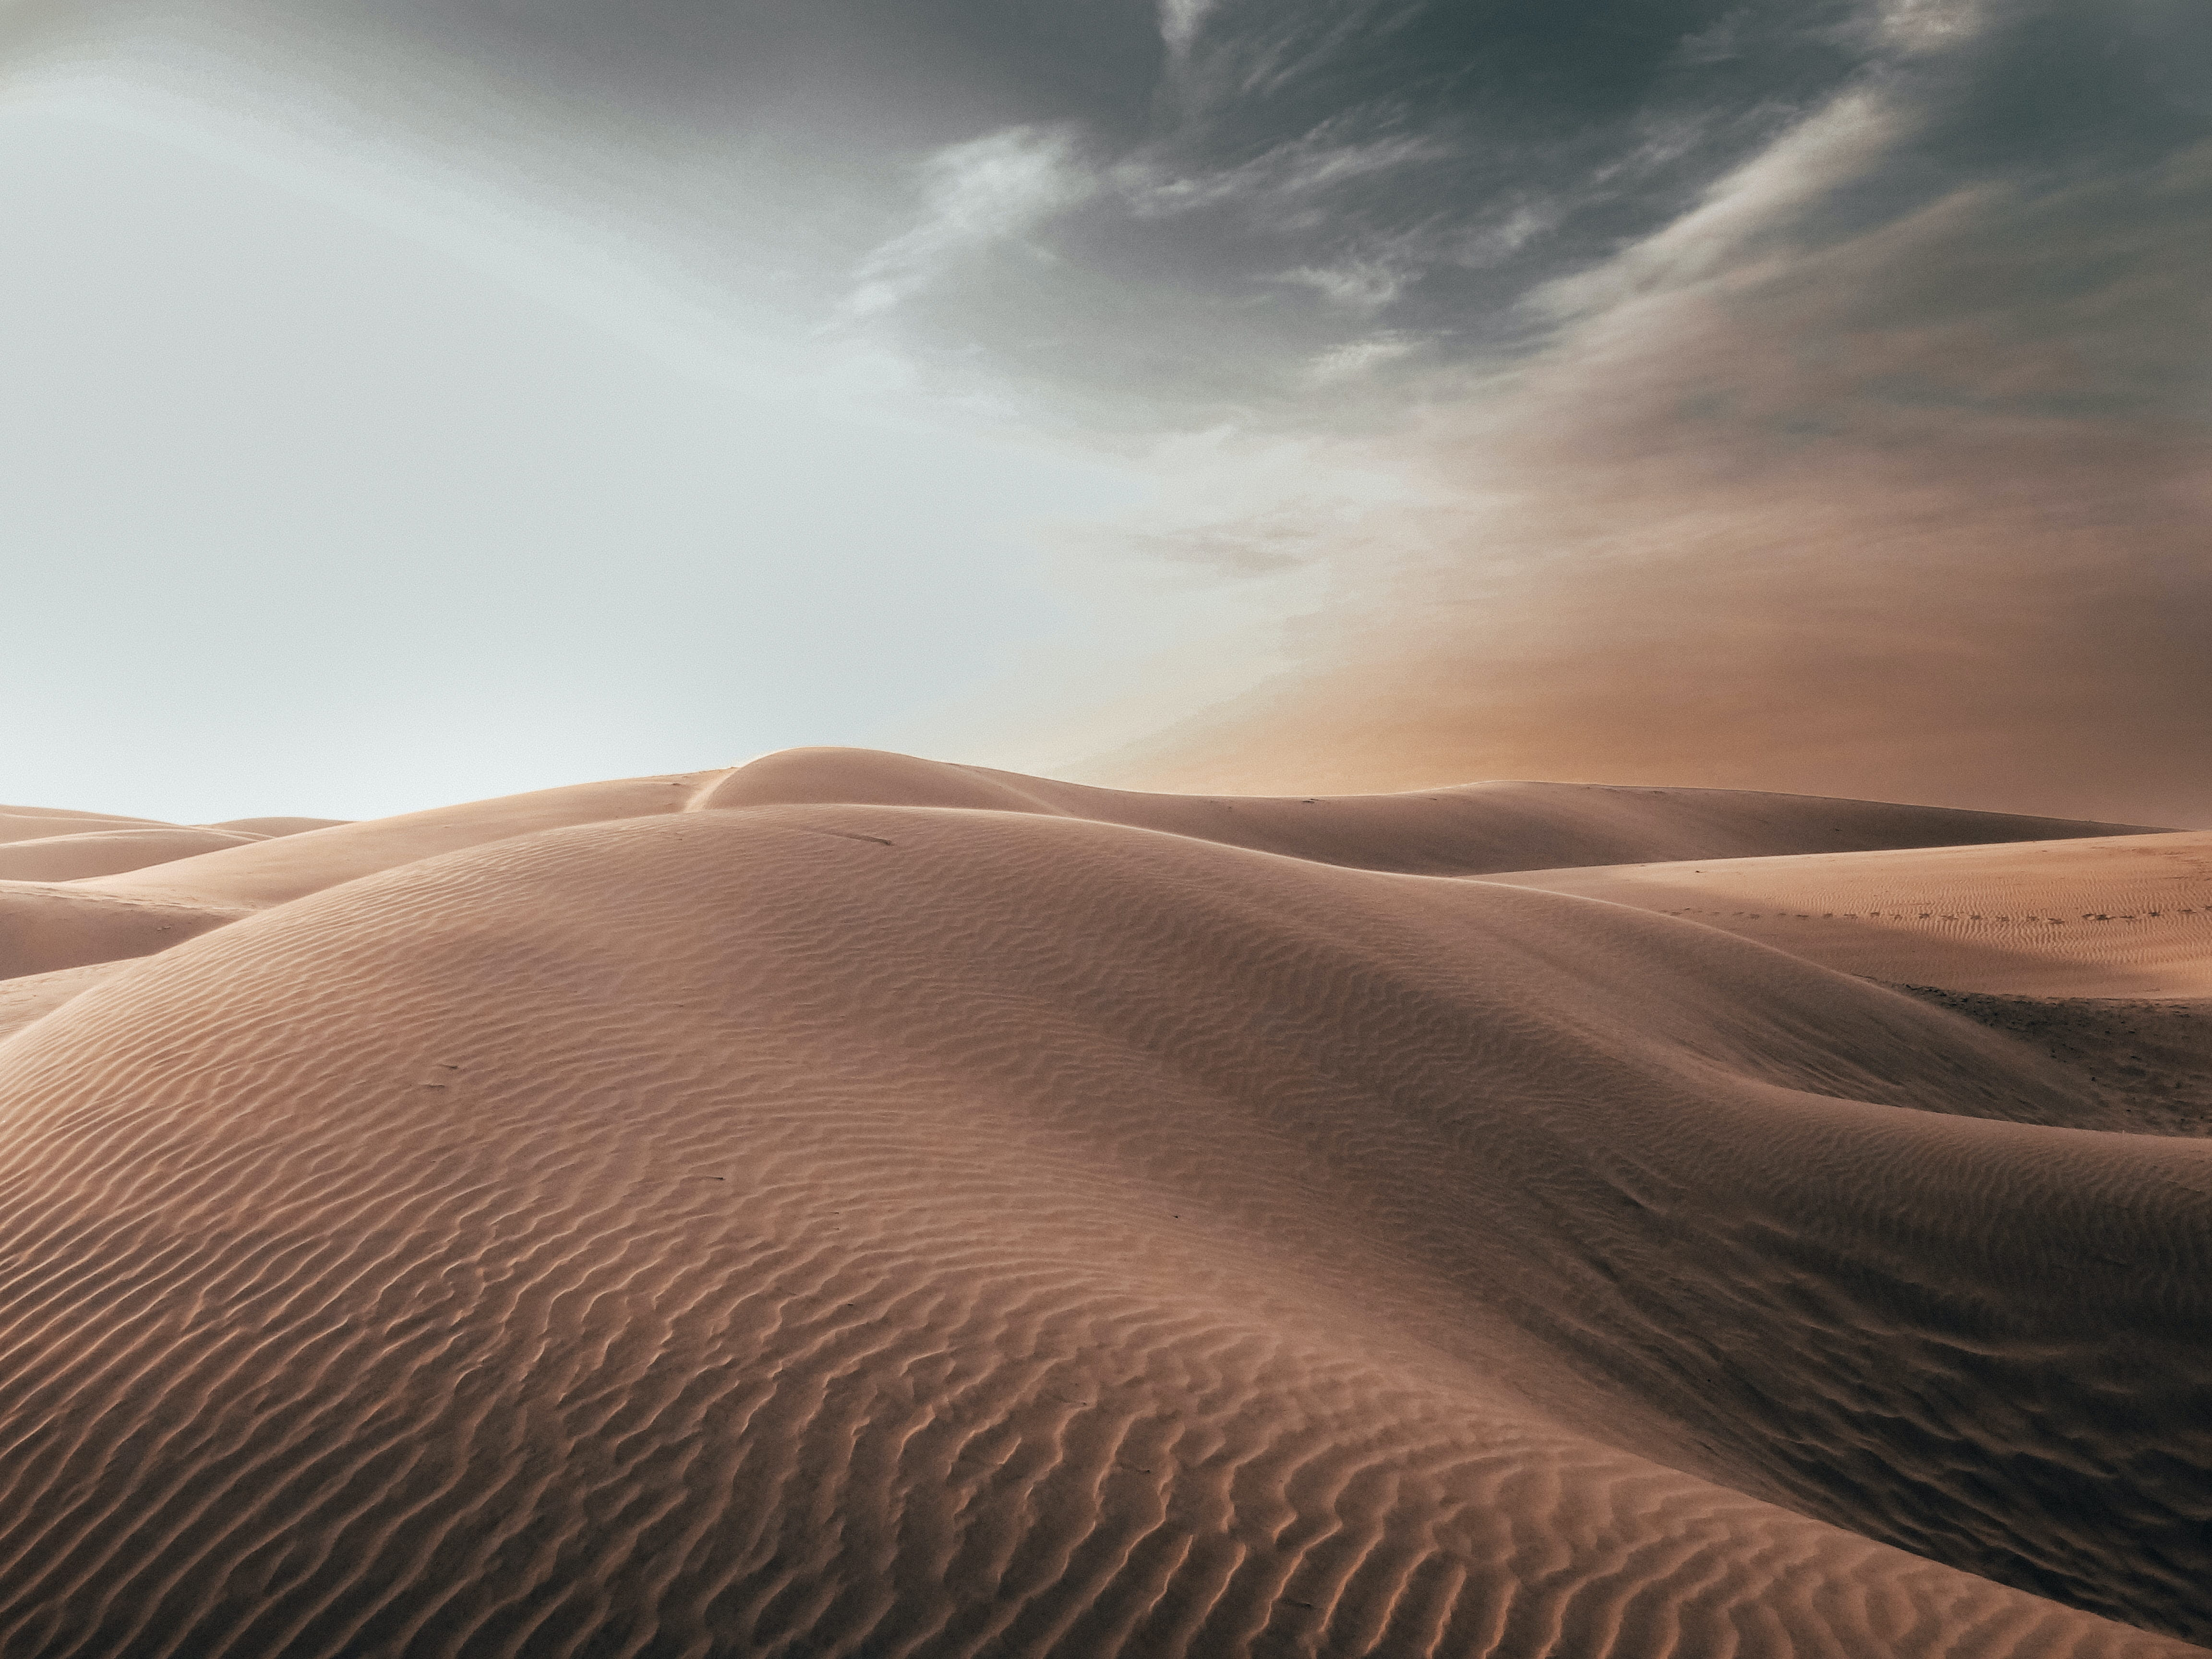
\includegraphics[width=\paperwidth]{duneslides-logo}}
\begin{frame}[plain,noframenumbering]

	\color{c++reviewduneblue}

	\begin{flushleft}\bfseries\scshape\huge
		Una introducción a la caja de herramientas Dune en
		C++/Python para la solución de modelos matemáticos
	\end{flushleft}

	\

	\

	\

	\

	\

	\

	\begin{minipage}{0.47\textwidth}
		\begin{figure}[ht!]
			\centering
			
\includegraphics[height=1.5cm]{alfaomega}
			\caption*{\large\bfseries\textcolor{c++reviewduneblue}{Webinar 12 de Julio de 2021}}
		\end{figure}
	\end{minipage}
	\begin{minipage}{0.5\textwidth}
		\begin{flushright}\large\bfseries
			Elaborado:\\
			John Jairo Leal Gómez\\
			Universidad Nacional de Colombia\\
			Carlos Alonso Aznarán Laos\\
			Universidad Nacional de Ingeniería, Perú
		\end{flushright}
	\end{minipage}

\end{frame}
}

%\frame[plain,noframenumbering]{\titlepage}
\section{Presentación del libro}

\begin{frame}
	\frametitle{\secname}%\hspace{-1cm}
	\begin{minipage}{0.47\textwidth}
		\begin{figure}[ht!]
			\centering
			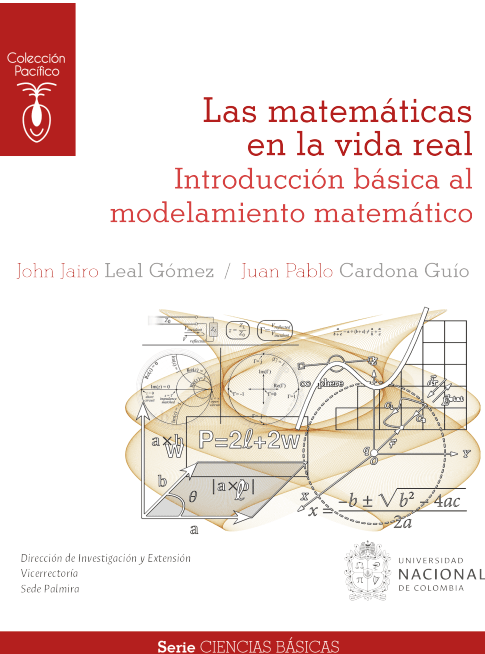
\includegraphics[height=7.7cm]{portada}
		\end{figure}
	\end{minipage}%\hspace{1cm}
	\begin{minipage}{0.5\textwidth}
		\textsc{\large Capítulos:}
		\begin{enumerate}
			\item Introducción a los números reales $\mathbb{R}$
			\item Introducción a las funciones
			\item La derivada
			\item Modelamiento matemático
			\item Anexos
		\end{enumerate}
	\end{minipage}

\end{frame}

\begin{frame}
	\frametitle{\secname}
	\begin{figure}[ht!]
		\centering
		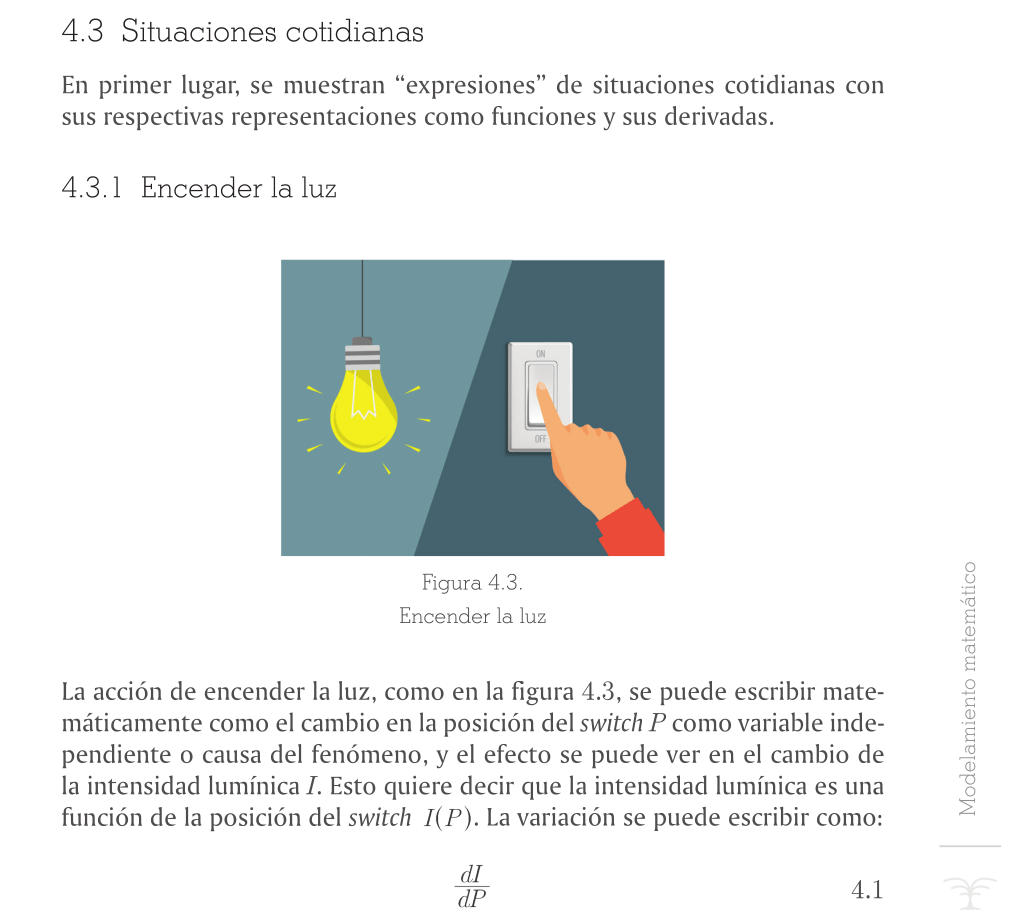
\includegraphics[height=7.7cm]{vida_cotidiana}
	\end{figure}
\end{frame}

\section{DUNE Numerics Project}
\subsection{Introducción}

\begin{frame}
	\frametitle{\secname}
	\framesubtitle{\subsecname}

	\begin{alertblock}{Distributed and Unified Numerics Environment (DUNE)}
		\note{Se hará una breve presentación de la caja de herramientas modular DUNE, biblioteca modular desarrollada en la universidad de Heildeberg Alemania en C++ y Python, para resolver ecuaciones diferenciales parciales utilizando métodos basados en mallas, por ejemplo diferencias finitas, elementos finitos o volúmenes finitos.}
		\begin{itemize}
			\item Software de código abierto bajo la licencia GNU General Public Licence 2.
			\item Disponible en \href{https://github.com/dune-copasi/homebrew-tap}{macOS}, Linux (Debian, Ubuntu  (\href{https://launchpad.net/~opm/+archive/ubuntu/ppa}{PPA}), OpenSUSE y Arch Linux) y freeBSD.
			      \note{Desarrollado con CMake, escrito en C++ con enlaces Python a través de pybind11.}
			\item Conjunto de bibliotecas C++ con enlaces a Python.
			\item Utilizado en la resolución de ecuaciones diferenciales parciales e implementación de métodos basados en mallas, por ejemplo diferencias finitas, elementos finitos o volúmenes finitos.
		\end{itemize}
		\note{Se mostrará la estructura general, proyectos basados en DUNE y algunas simulaciones de modelos matemáticos que incluyen éste tipo de ecuaciones, así como una implementación breve de DUNE.}
	\end{alertblock}

	\

	\begin{figure}[ht!]
		\centering
		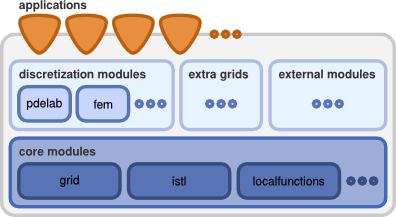
\includegraphics[height=4cm]{dunedesign}
		\caption{Tomado de \url{https://dune-project.org}}
	\end{figure}

\end{frame}

\begin{frame}
	\frametitle{\secname}
	\framesubtitle{\subsecname}

	\begin{columns}
		\begin{column}{0.5\textwidth}
			\begin{alertblock}{Proyectos que emplean DUNE}
				\begin{itemize}
					\item \url{https://dune-project.org/about/dune}
					\item \url{https://dumux.org}
					\item \url{https://opm-project.org}
					\item \url{https://www.zib.de/projects/kaskade7-finite-element-toolbox}
				\end{itemize}
			\end{alertblock}
		\end{column}

		\begin{column}{0.5\textwidth}
			\begin{figure}[ht!]
				\centering
				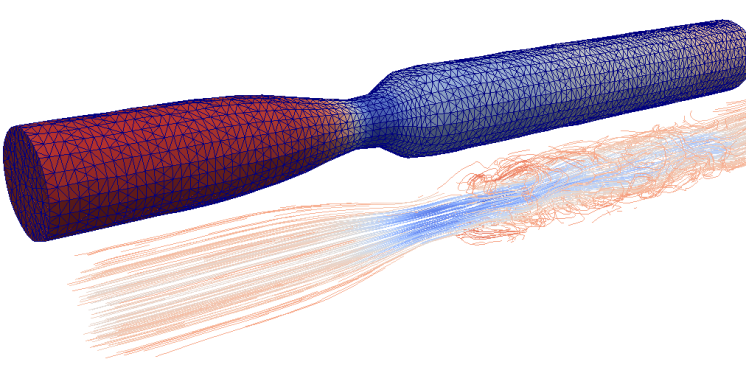
\includegraphics[width=7cm]{blood_girke}
				\caption{Tomado de \url{https://dune-project.org}}
			\end{figure}
		\end{column}
	\end{columns}
\end{frame}

\section{Curso de DUNE/PDELab (8/3/2021 - 12/3/2021)}

\begin{frame}[fragile]
	\frametitle{\secname}
	\framesubtitle{\url{https://dune-pdelab-course.readthedocs.io}}

	\begin{figure}[ht!]
		\centering
		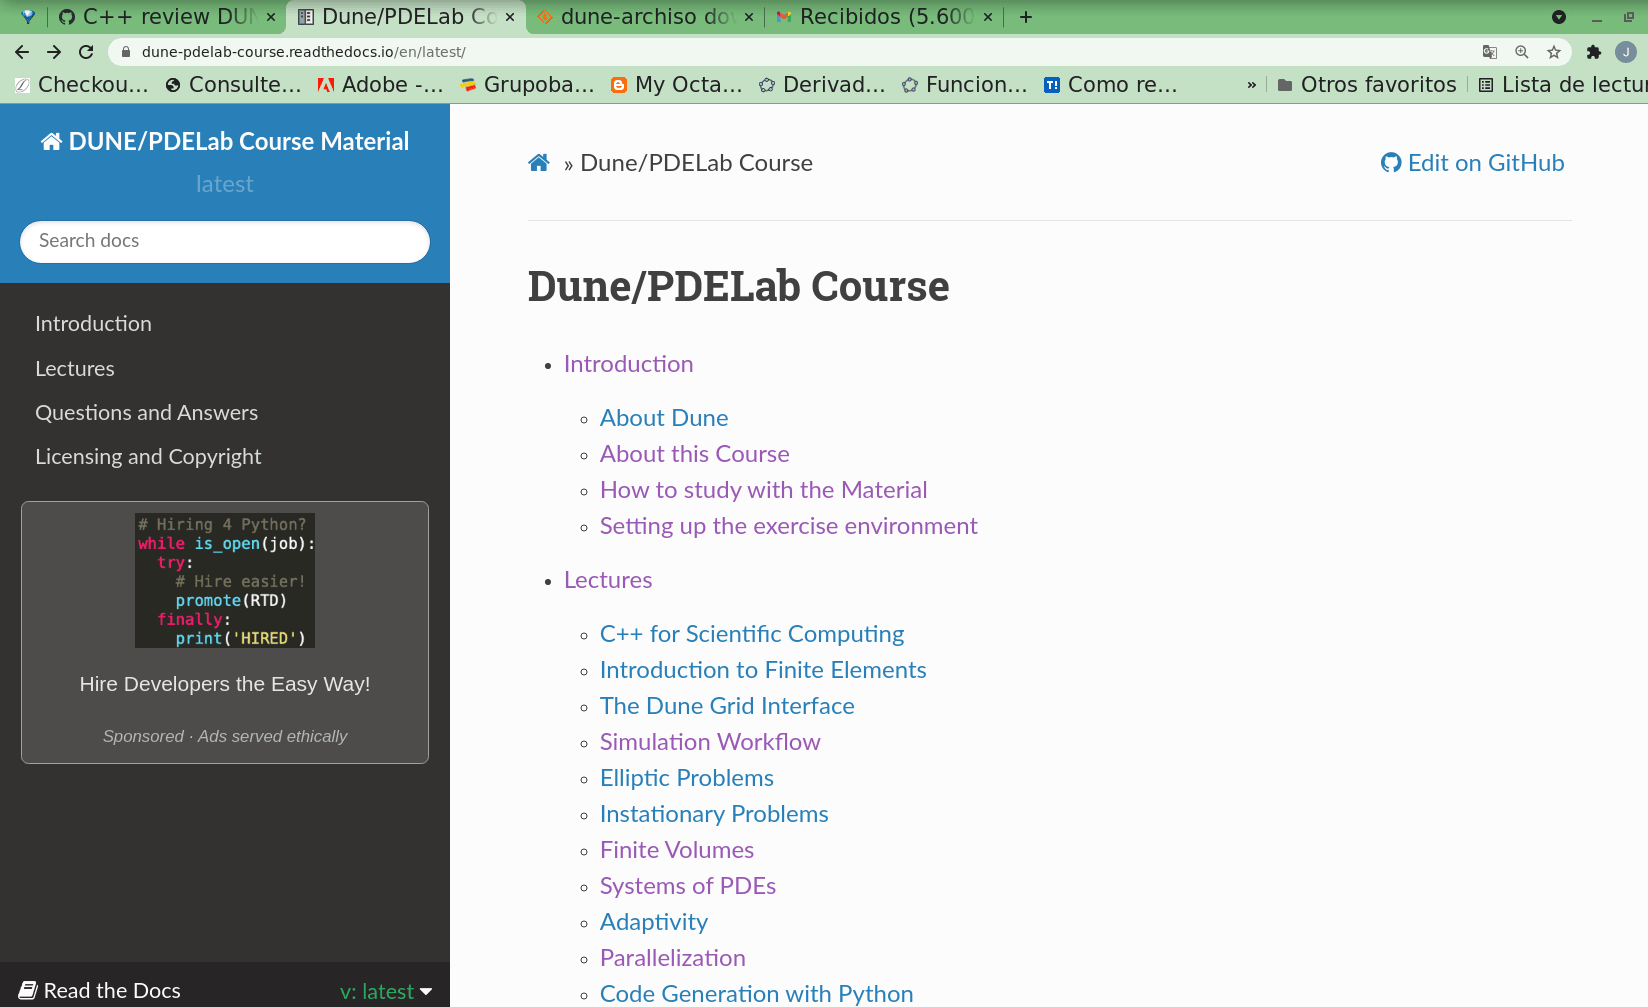
\includegraphics[height=8cm]{dune_course_2021}
	\end{figure}
	\note{Cursos de DUNE anuales, lista de correo de preguntas y noticias}
\end{frame}

\begin{frame}[fragile]
	\frametitle{\secname}
	\framesubtitle{Snippet en C++}
	\lstinputlisting[caption={Programa \texttt{dune-basics.cc}.},label=dune-basics.cc,]{dune-basics.cc}
\end{frame}

\begin{frame}[fragile]
	\frametitle{\secname}
	\framesubtitle{Snippet en Python}
	\lstinputlisting[caption={Programa \texttt{dune-basics.cc}.},label=dune-basics.cc,]{dune-basics.cc}
\end{frame}

{
\usebackgroundtemplate{\centering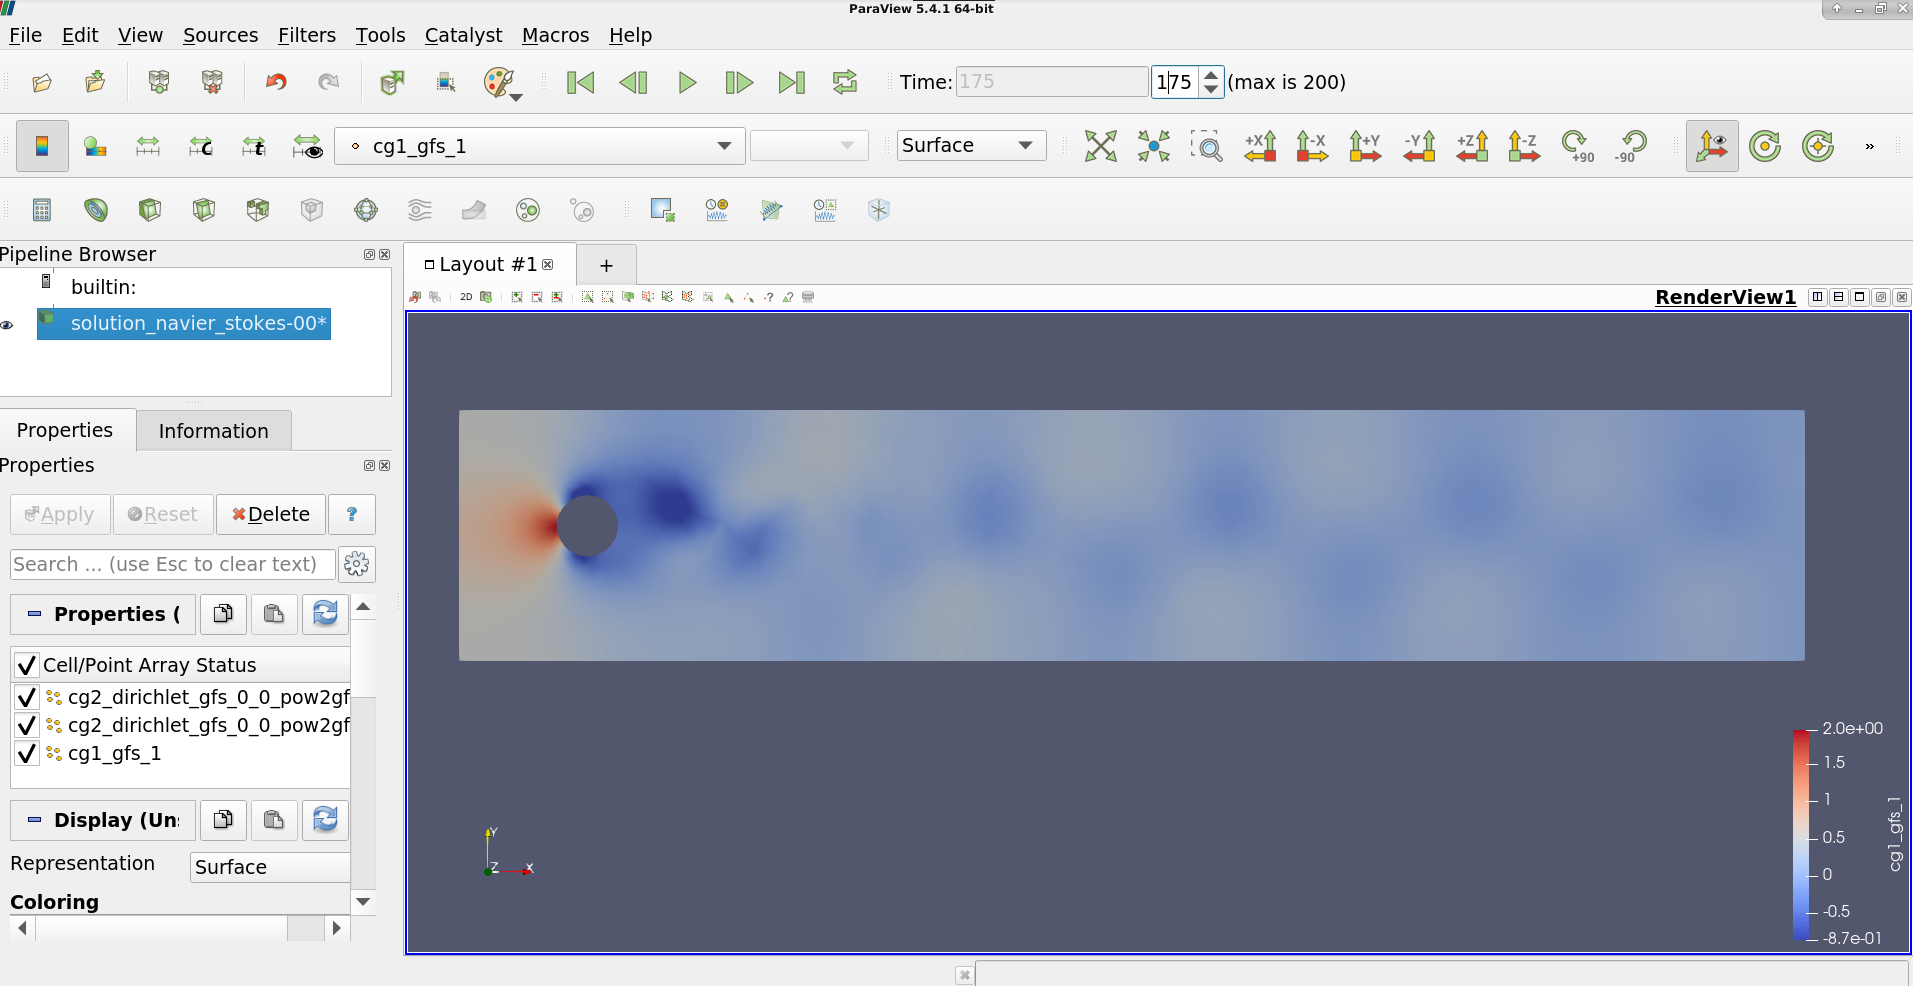
\includegraphics[width=\paperwidth]{tutorial-9}}
\begin{frame}[plain]
\end{frame}
}

{
\usebackgroundtemplate{\centering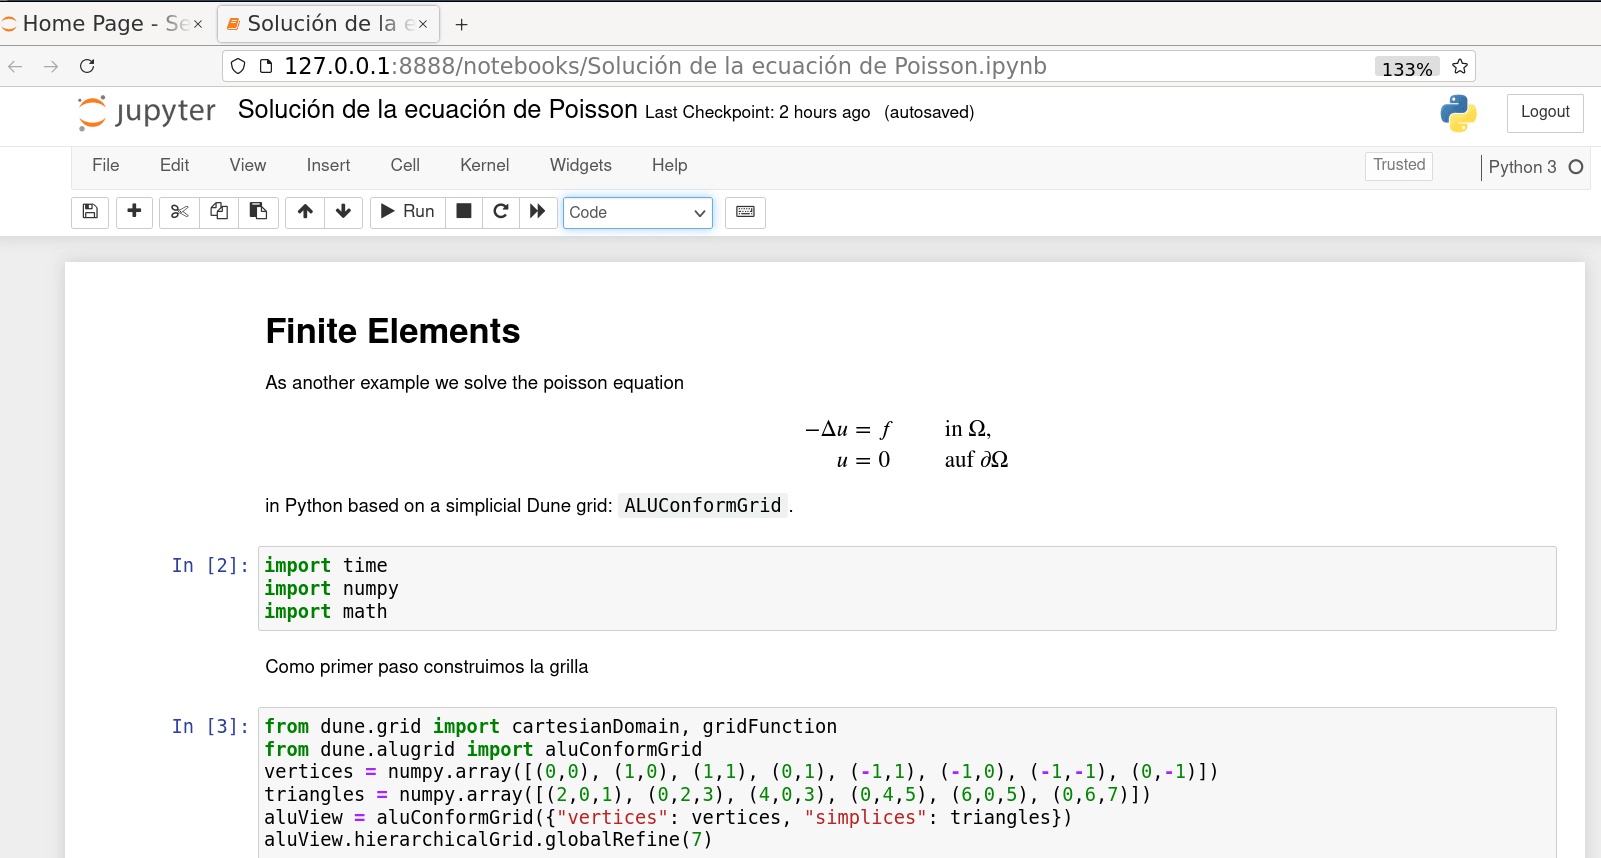
\includegraphics[width=\paperwidth]{jupyter01}}
\begin{frame}[plain]
\end{frame}
}
\section{DUNE Latinoamérica}
\begin{frame}
	\frametitle{\secname}
	\framesubtitle{Página para revisión de DUNE}
	\begin{figure}[ht!]
		\centering
		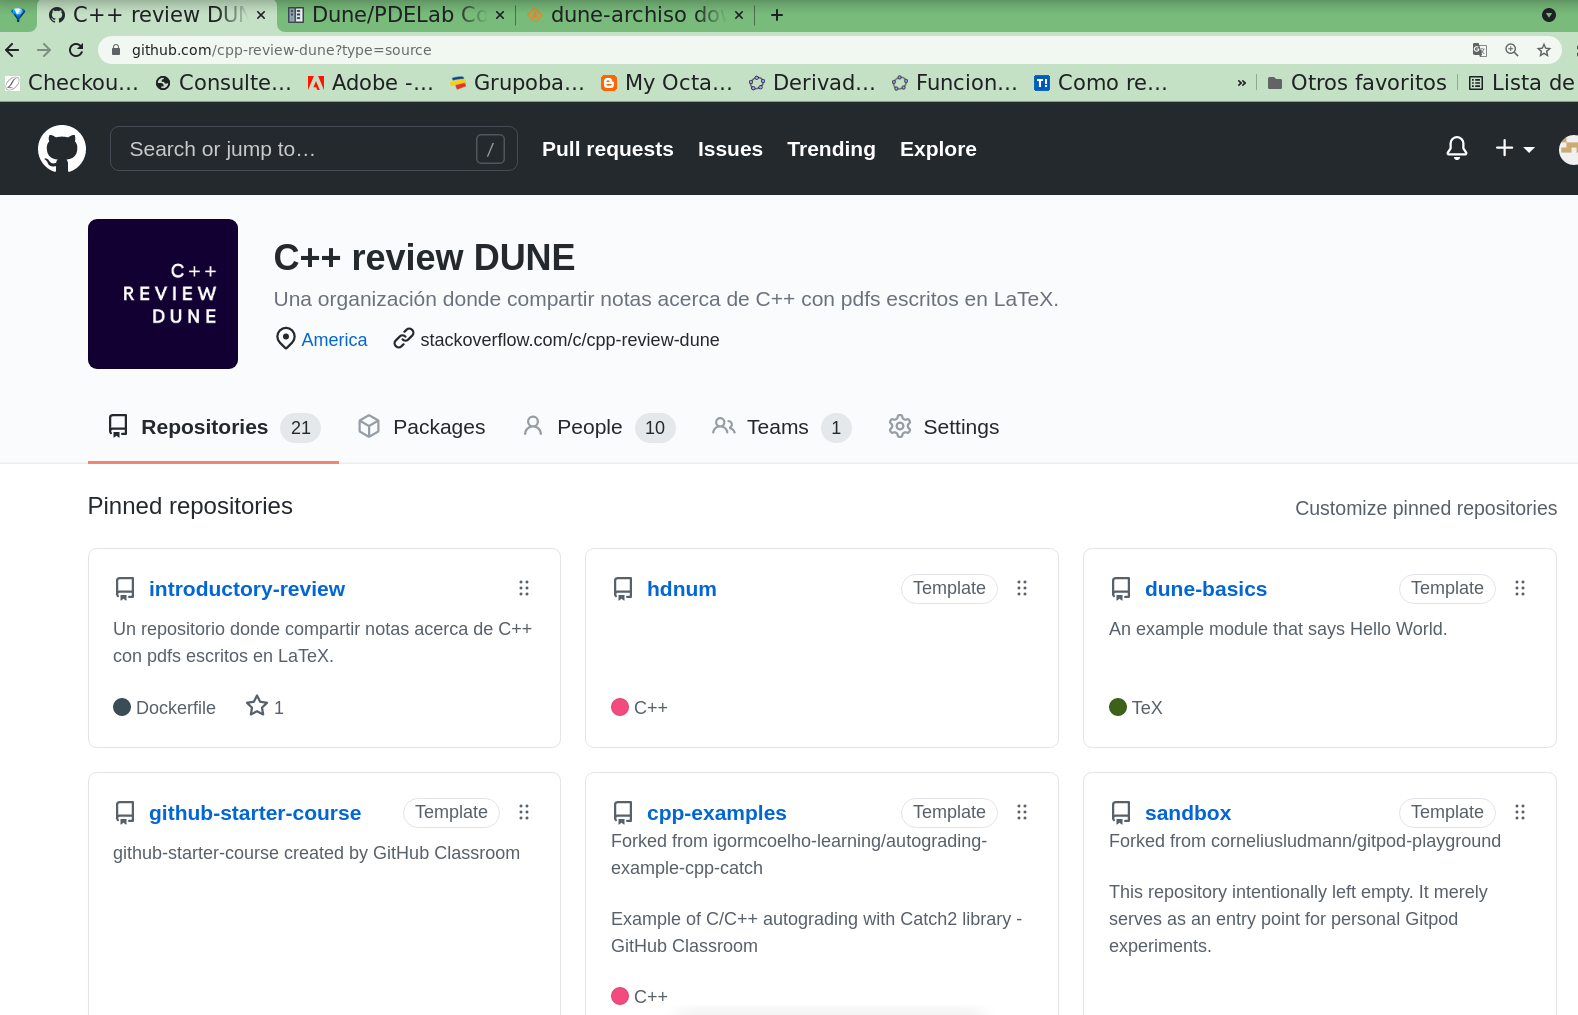
\includegraphics[height=8cm, width=12cm]{cpp_review}
	\end{figure}
\end{frame}

\begin{frame}
	\frametitle{\secname}
	\framesubtitle{Imágenes Docker en Achlinux}
	\begin{figure}[ht!]
		\centering
		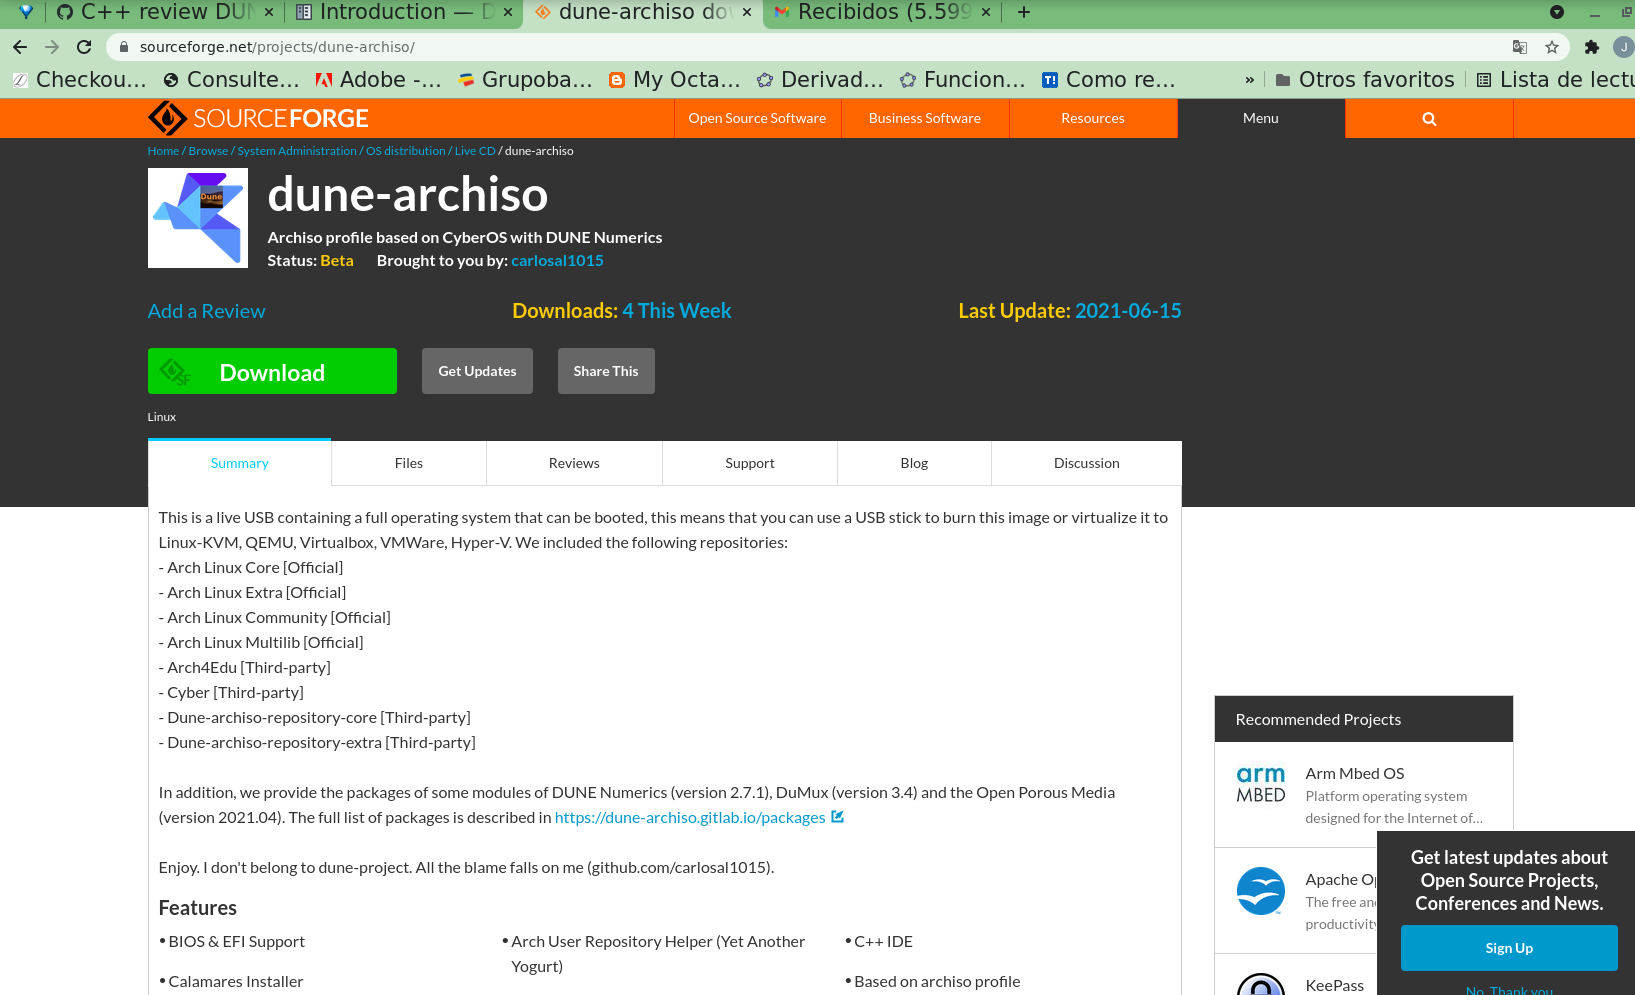
\includegraphics[height=8cm, width=12cm]{archiso}
	\end{figure}
\end{frame}

\subsection{Módulos}

\begin{frame}
	\frametitle{\secname}
	\framesubtitle{\subsecname}

	\begin{columns}
		\begin{column}{0.5\textwidth}
			\dirtree{%
				.1 dune-fem.
				.2 dune-grid.
				.3 dune-geometry.
				.4 dune-common.
			}

			\

			\

			\dirtree{%
				.1 dumux.
				.2 dune-istl.
				.2 dune-localfunctions.
				.2 vc.
				.2 psurface.
				.2 superlu.
				.2 arpack++.
				.2 suitesparse.
				.2 dune-alugrid.
				.2 dune-subgrid.
				.2 fmt.
				.2 opm-common.
			}
		\end{column}

		\begin{column}{0.5\textwidth}
			\dirtree{%
				.1 opm-upscaling.
				.2 opm-grid.
				.3 opm-common.
				.4 dune-grid.
				.5 dune-geometry.
				.4 dune-istl.
				.4 boost.
			}

			\

			\

			\dirtree{%
				.1 opm-models.
				.2 opm-material.
				.3 opm-common.
				.4 dune-grid.
				.5 dune-geometry.
				.4 dune-istl.
				.4 boost.
			}
		\end{column}
	\end{columns}

\end{frame}
\subsection{El DUNE verso: módulos}
\begin{frame}
	\frametitle{\secname}
	\framesubtitle{\subsecname}

	\begin{figure}[ht!]
		\centering
		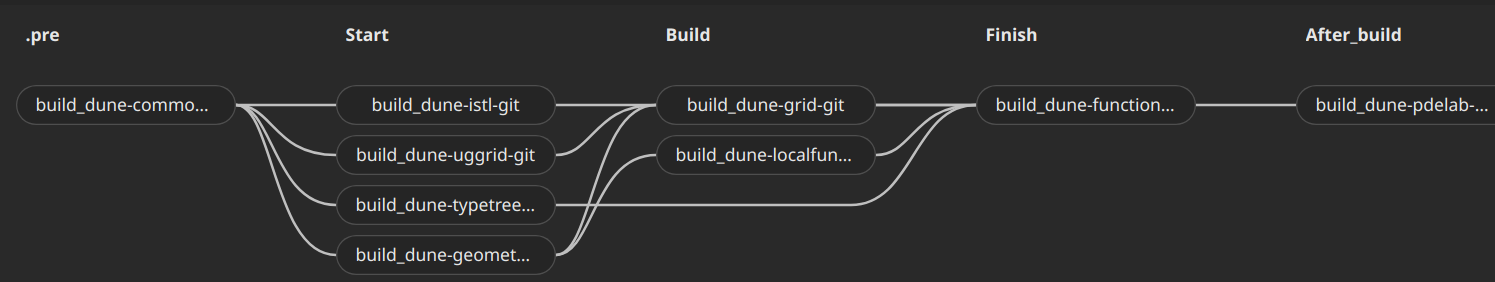
\includegraphics[width=14.5cm]{dependences}
	\end{figure}

	\begin{description}
		\item[dune-common]

		Clases fundamentales e infraestructura para la construcción del sistema.

		\note{contiene las clases base usadas por todos los módulos de DUNE-modules. Provee algunas clases de infraestructura para depuración y manejo de excepciones así como una librería para manejar una matriz densa.
and vectors.}

		\item[dune-geometry] Elementos de referencia, métodos de cuadratura y transformaciones geométricas.

		\item[dune-grid] Interfaces con las mallas (ALUGrid, UGGrid, Alberta, YasGrid), construcción y visualización.

		\item[dune-istl] Biblioteca de solucionadores iterativas de plantillas, clases genéricas de matrices/vectores dispersos, solucionadores

		\item[dune-localfunctions] Interface genérica para funciones de elementos finitos.
	\end{description}
\end{frame}

\begin{frame}\transblindsvertical
	\frametitle{Referencias}
	%------------------------------------------------------------ 1
	\only<1>{
		\begin{itemize}
			\item Libros
			      \nocite{*}
			      \printbibliography[heading=none,keyword=book]
		\end{itemize}
	}
	%------------------------------------------------------------ 2
	\only<2>{
		\begin{itemize}
			\item Artículos
			      \printbibliography[heading=none,keyword=paper]
		\end{itemize}
	}
	%------------------------------------------------------------ 3
	\only<3>{
		\begin{itemize}
			\item Sitios web
			      \printbibliography[heading=none,keyword=online]
		\end{itemize}
	}
\end{frame}

\end{document}
%https://conan.iwr.uni-heidelberg.de/events/dune-course_2021/